Die Gesetze der Bewegung, auch Translation genannt, ist ein wiederkehrendes Thema in der Physik. Die Gesetze beschreiben die Bewegung von Körpern und geben deren Ort in Abhängigkeit einer Variablen, meistens der Zeit, an:

\subsection{Gleichförmige Bewegung} \label{subsec:gleichfoermig}

Die gleichförmige Bewegung ist eine Bewegung, die nicht beschleunigt ist; der Körper bewegt sich mit einer konstanten Geschwindigkeit fort. Daher gilt für die insgesamt zurückgelegte Strecke $s$:

\begin{align} \label{eq:gleichfoermig}
	s(t) = v \cdot t + s_0
\end{align}

\begin{figure}[h!]
	\centering
	\begin{minipage}[b]{0.45\linewidth}
		\begin{comment} Gnuplot:
set xlabel "t"
set ylabel "s(t)"
set output "plot_bewegung_gleichfoermig_s.png"
plot s(x) = 1x ls 1
		\end{comment}
    	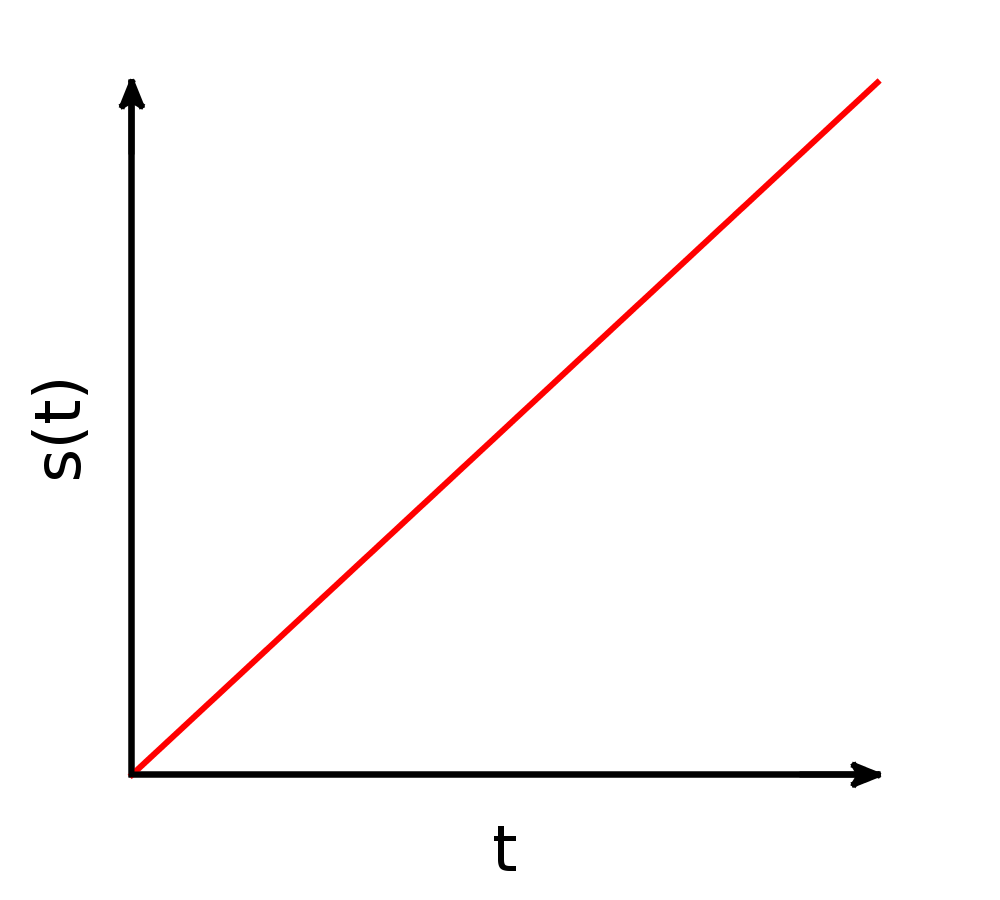
\includegraphics[width=\textwidth]{plot_bewegung_gleichfoermig_s}
	\end{minipage}
	\begin{minipage}[b]{0.45\linewidth}
		\begin{comment} Gnuplot:
set xlabel "t"
set ylabel "v(t)"
set output "plot_bewegung_gleichfoermig_v.png"
plot 1 ls 1
		\end{comment}
    	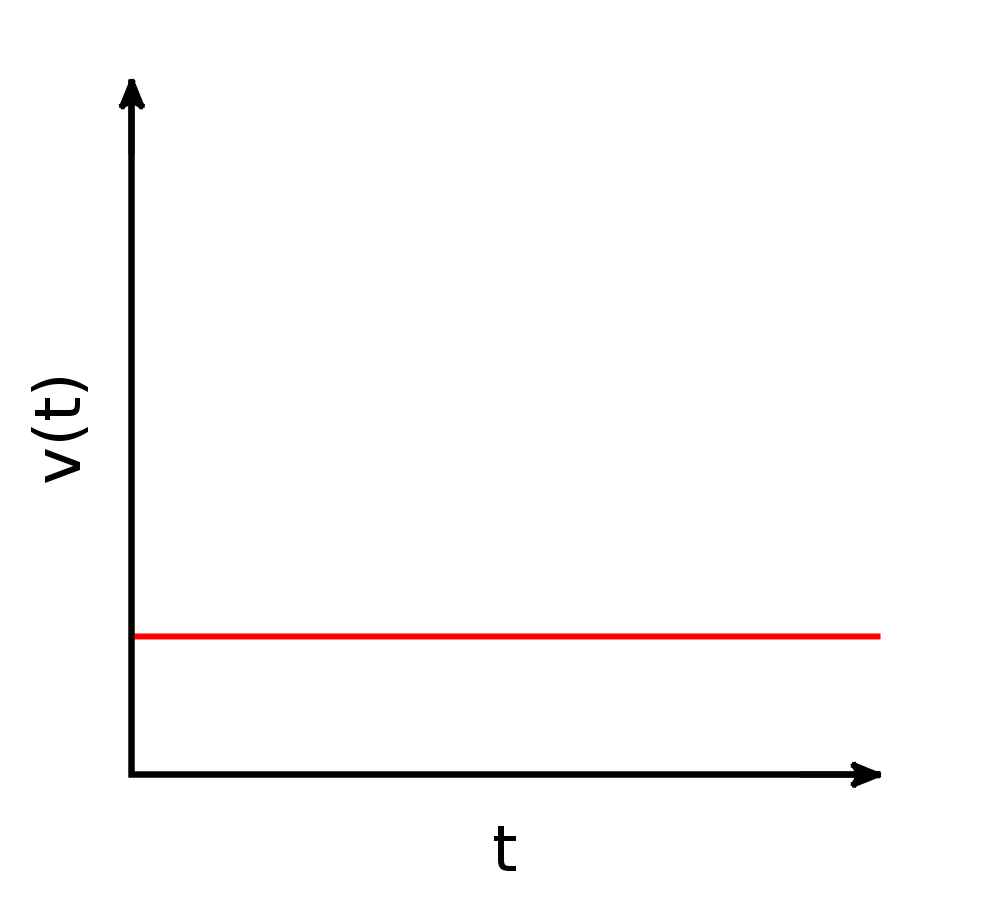
\includegraphics[width=\textwidth]{plot_bewegung_gleichfoermig_v}
	\end{minipage}
	\caption{Gleichförmige Bewegung: Beziehung zwischen Weg und Geschwindigkeit}
	\label{fig:gleichfoermig}
\end{figure}


\begin{Wichtig}
$v$ ist konstant!
\end{Wichtig}

\noindent Dabei ist $s_0$ die Anfangsstrecke, die schon zu Beginn, bevor die Translation betrachtet wird, zurückgelegt wurde.

\begin{figure}[h!]
	\centering
	\begin{comment} Gnuplot:
set xlabel "t"
set ylabel "s(t)+s_0"
set output "plot_bewegung_gleichfoermig_s+s0.png"
plot s(x) = 1x+1 ls 1
	\end{comment}
	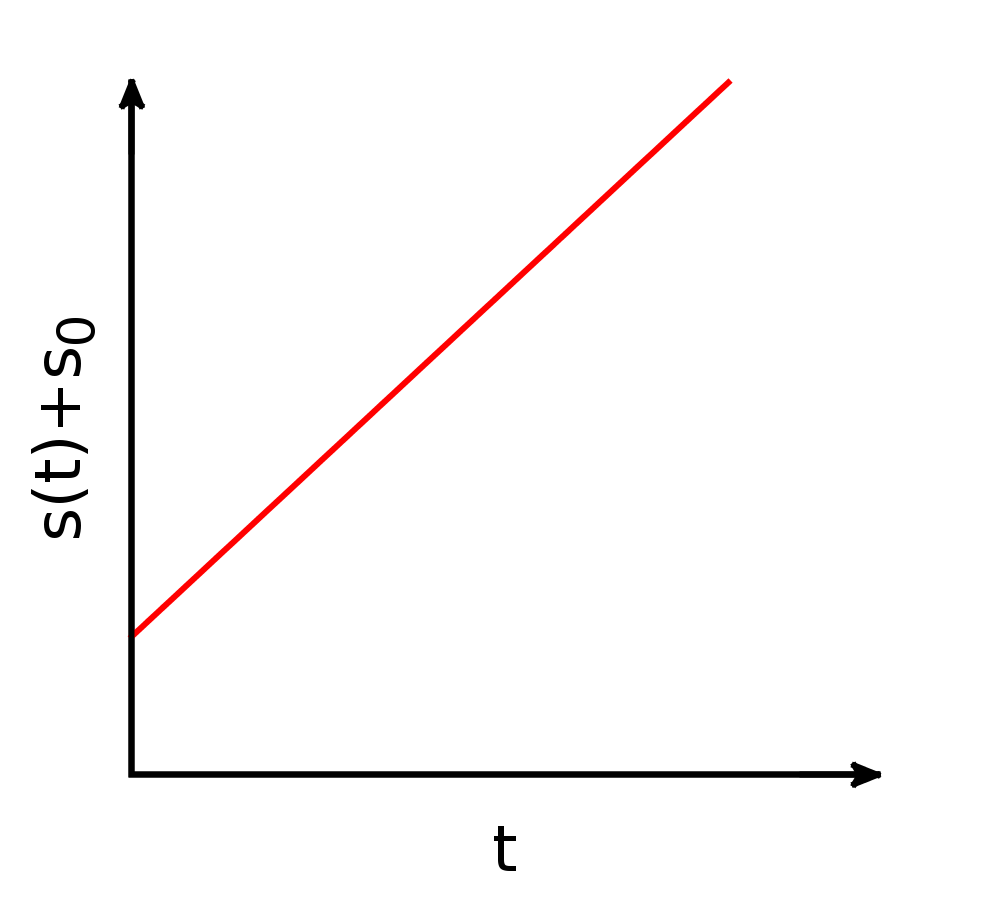
\includegraphics[width=0.6\textwidth]{plot_bewegung_gleichfoermig_s+s0}
	\caption{Mit Anfangsgeschwindigkeit: Der Graph ist verschoben}
\end{figure}

\subsection{Gleichmäßig beschleunigte Bewegung}

Eine Bewegung kann auch mit einer sich ändernden Geschwindigkeit von statten gehen. Sollte diese Beschleunigung konstant sein, nennt man diese Bewegung gleichmäßig beschleunigte Bewegung.

\subsubsection{Gesamtstrecke}

Bei dieser Bewegung lässt sich die Durchschnittsgeschwindigkeit über den Zeitraum $t$ mit $\frac{1}{2}a \cdot t$ berechnen, da die Endgeschwindigkeit $a \cdot t$ ist: Die Änderung der Geschwindigkeit $a$, angewandt über den Zeitraum $t$, resultiert in der Endgeschwindigkeit. Da die Beschleunigung konstant ist und damit die Geschwindigkeit proportional zur Zeit, ist der Faktor, der zur gemittelten Geschwindigkeit führt $\frac{1}{2}$.

Dann kann dieses $\frac{1}{2}a \cdot t$ für das $v$ im ersten Glied der Gleichung \ref{eq:gleichfoermig} eingesetzt werden und man erhält die Bewegungsgleichung für die gleichmäßig beschleunigte Bewegung:

\begin{align} \label{eq:streckegleichmaessig}
	s(t) = \frac{1}{2}a \cdot t^2 + v_0 \cdot t + s_0
\end{align}

\begin{figure}[h!]
	\centering
	\begin{minipage}[b]{0.32\linewidth}
		\begin{comment} Gnuplot:
set xlabel "t"
set ylabel "s(t)"
set output "plot_bewegung_beschleunigt_s.png"
plot 0.5 * 1 * x * x ls 1
		\end{comment}
    	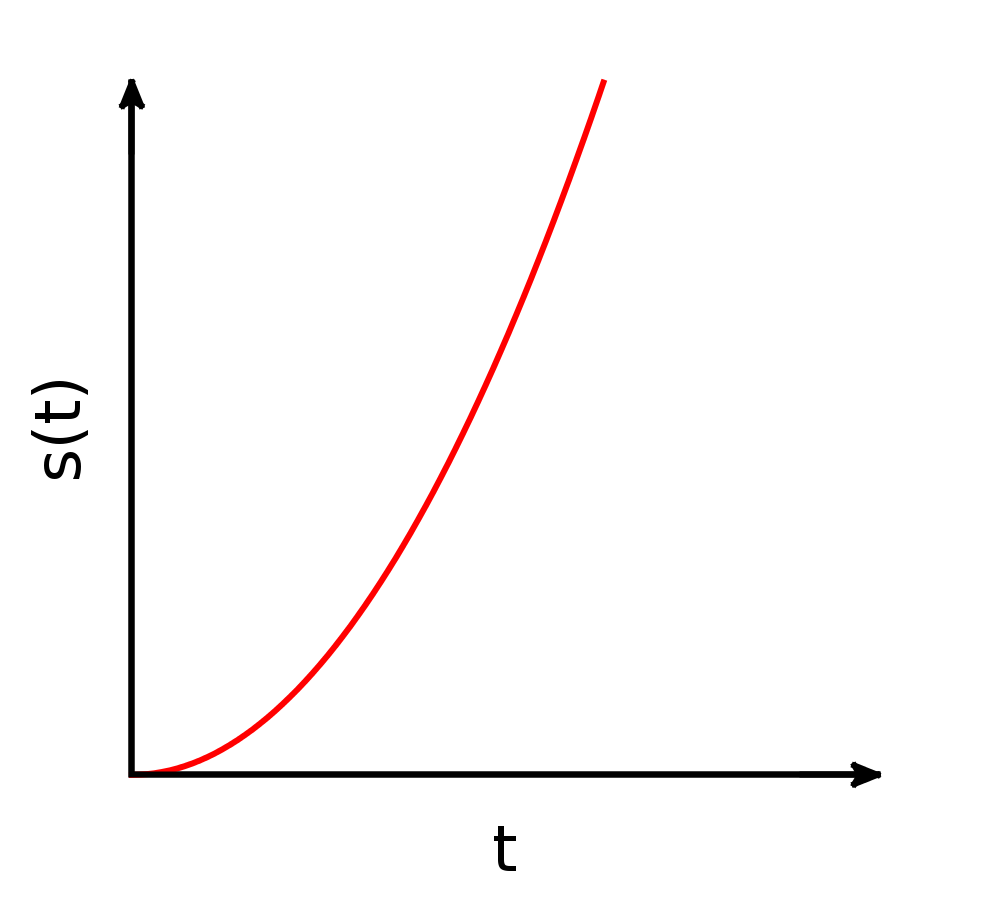
\includegraphics[width=\textwidth]{plot_bewegung_beschleunigt_s}
	\end{minipage}
	\begin{minipage}[b]{0.32\linewidth}
		\begin{comment} Gnuplot:
set xlabel "t"
set ylabel "v(t)"
set output "plot_bewegung_beschleunigt_v.png"
plot x ls 1
		\end{comment}
    	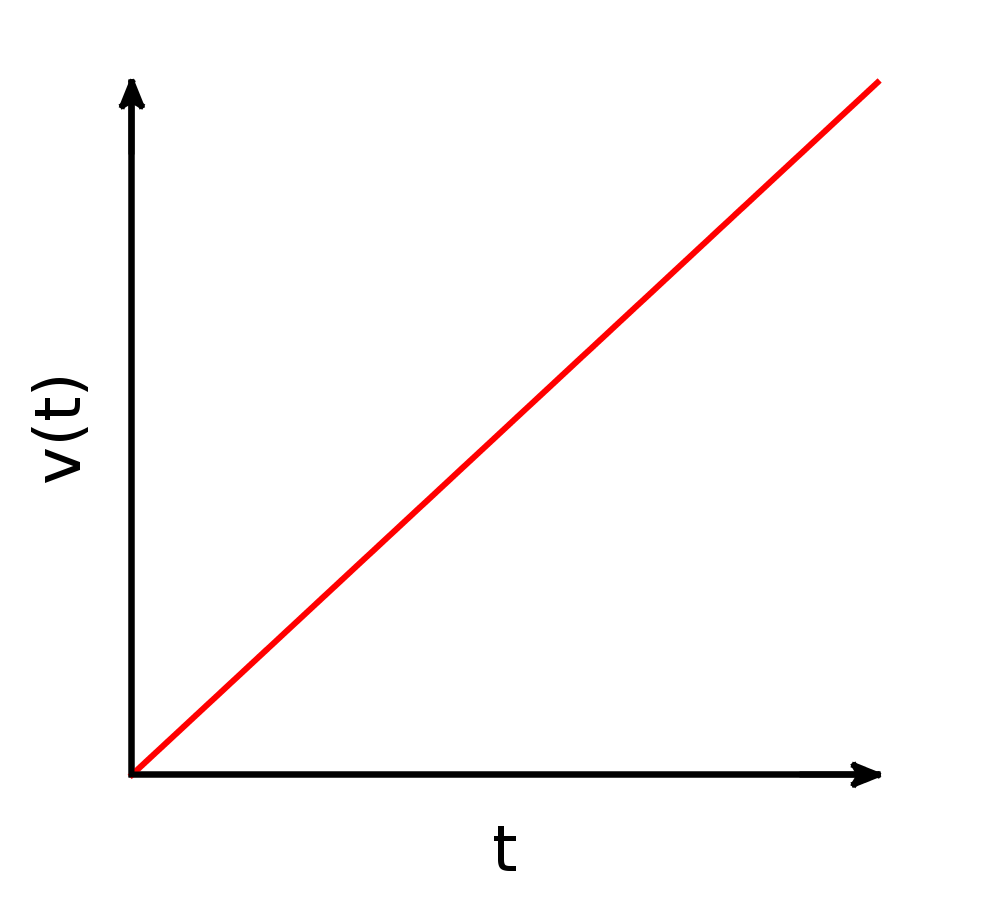
\includegraphics[width=\textwidth]{plot_bewegung_beschleunigt_v}
	\end{minipage}
	\begin{minipage}[b]{0.32\linewidth}
		\begin{comment} Gnuplot:
set xlabel "t"
set ylabel "a(t)"
set output "plot_bewegung_beschleunigt_a.png"
plot 1 ls 1
		\end{comment}
    	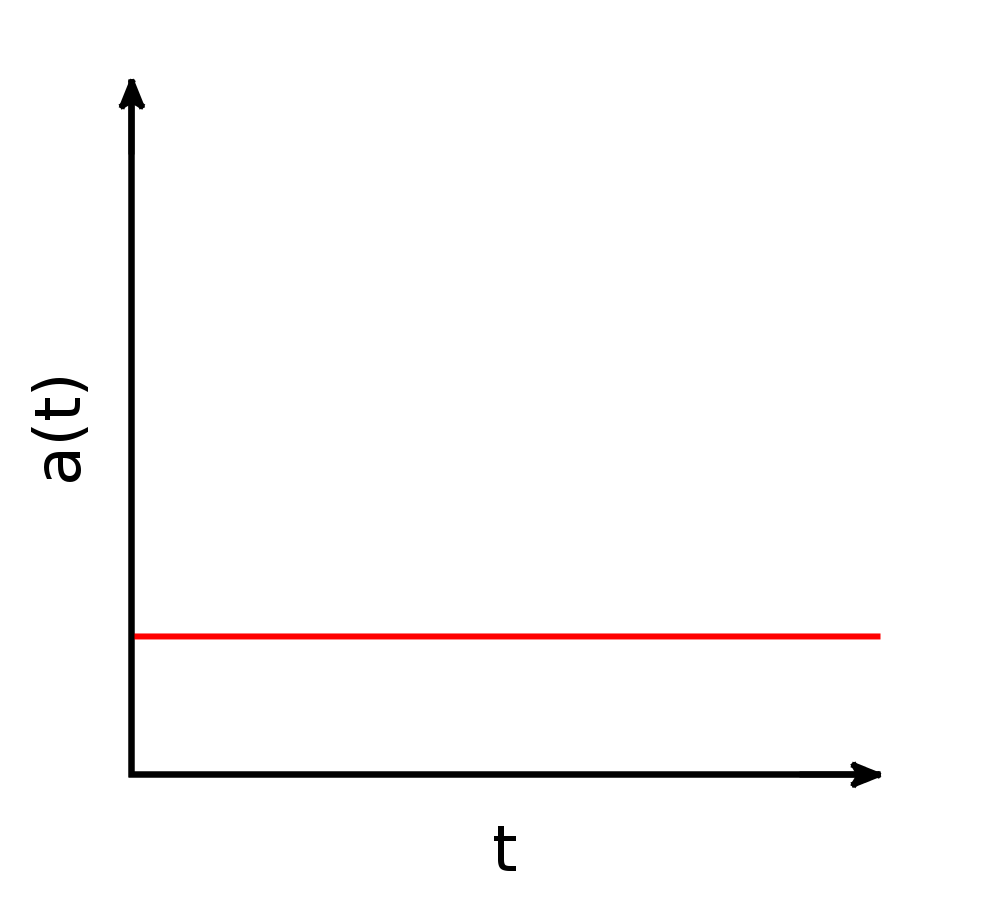
\includegraphics[width=\textwidth]{plot_bewegung_beschleunigt_a}
	\end{minipage}
	\caption{Gleichmäßig beschleunigte Bewegung: Beziehung zwischen Weg, Geschwindigkeit und Beschleunigung}
	\label{fig:beschleunigt}
\end{figure}

\noindent Neben der Anfangsstrecke $s_0$ kommt nun aber auch noch die Anfangsgeschwindigkeit $v_0$ dazu, die von Belang ist, wenn man einen Fall hat, bei dem der Körper vor Einwirkung der Beschleunigung schon eine Geschwindigkeit $>0$ hatte.


\subsubsection{Endgeschwindigkeit}

Wie schon angesprochen, ist die Endgeschwindigkeit proportional zur verstrichenen Zeit. Was aber dort noch nicht berücksichtigt wurde, ist, dass auch für die Endgeschwindigkeit nach der verstrichenen Zeit $t$ die Anfangsgeschwindigkeit $v_0$ eine Rolle spielt:

\begin{align}	\label{eq:geschwindigkeitgleichmaessig}
	v(t) = a \cdot t + v_0
\end{align}

\noindent Dies ist die zeitliche Ableitung der Gleichung \ref{eq:streckegleichmaessig}


\subsubsection{Beziehungen über die Ableitungen}

Würde man noch eine Ableitung der Gleichung \ref{eq:geschwindigkeitgleichmaessig} machen bekäme man die Gleichung für die Beschleunigung. Das wäre aber witzlos, da die Beschleunigung einer gleichmäßig beschleunigten Bewegung konstant ist und damit $s''(t)=v'(t)=a(t)=a= const.$ ist. Vergleiche mit Abbildung \ref{fig:beschleunigt}\endnote{Abbildungen \ref{fig:gleichfoermig}-\ref{fig:beschleunigt}: \glqq Translationsdiagramme\grqq{} von Till Blaha - Eigene Werke. Lizenziert unter Gemeinfrei.}.

Dennoch ist es hilfreich, diese Beziehungen im Kopf zu haben (Man beziehe auch Abbildung \ref{fig:beschleunigt}):

\begin{align}
\begin{split}
	s'(t) &= v(t) \\
	v'(t) &= a \\
	s''(t) &= v'(t)= a
\end{split}
\end{align}

\noindent Die Ableitung des Weges, also die zeitliche Änderung des Weges, ist die Geschwindigkeit. Die zeitliche Änderung der Geschwindigkeit ist die Beschleunigung. Daher ist die zeitliche Änderung der zeitlichen Änderung des Weges, die Beschleunigung.



